\pagebreak
\section{Introduction}
\label{sec:introduction}

% state the learning objective 
The objective of this laboratory assignment is to study a circuit containing one independent and one dependent voltage sources, $V_a$ and $V_c$ respectively, as well as one independent and one dependent current sources, $I_d$ and $I_b$, connected to 7 resistors. The circuit can be seen in Figure~\ref{fig:circuito_t1}.



In Section~\ref{sec:analysis}, a theoretical analysis of the circuit is
presented. In Section~\ref{sec:simulation}, the circuit is analysed by
simulation, and the results are compared to the theoretical results obtained in
Section~\ref{sec:analysis}. The conclusions of this study are outlined in
Section~\ref{sec:conclusion}.

\begin{figure}[H] \centering
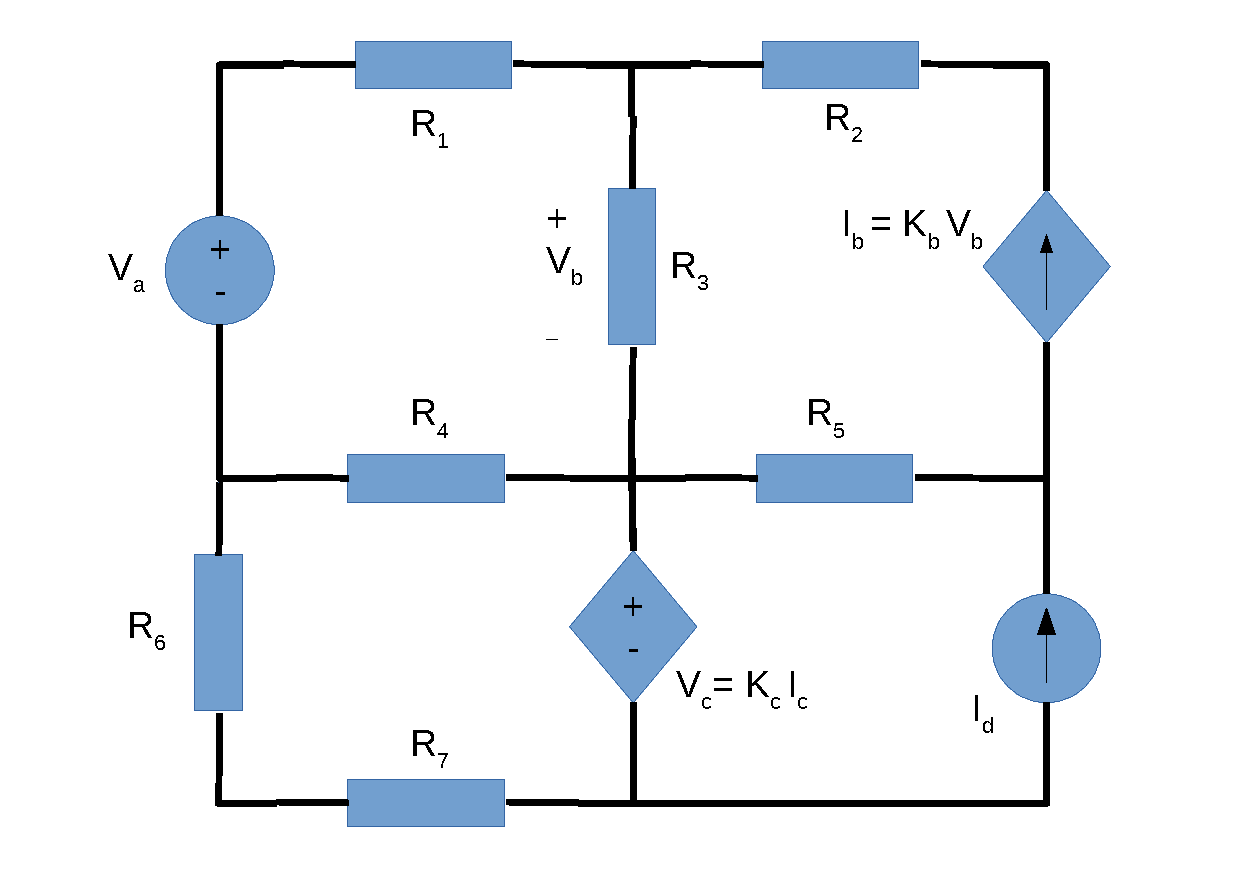
\includegraphics[width=0.5\linewidth]{circuito_T1.pdf}
\caption{Circuit for Lab T1.}
\label{fig:circuito_t1}
\end{figure}

